\begin{figure}[h!]
    \begin{center}
    \caption{Effects on Infant Mortality Rates}\label{fig:15}
    \begin{subfigure}{0.32\textwidth}
        \caption{\scriptsize Total}\label{fig:15a}
        \centering
        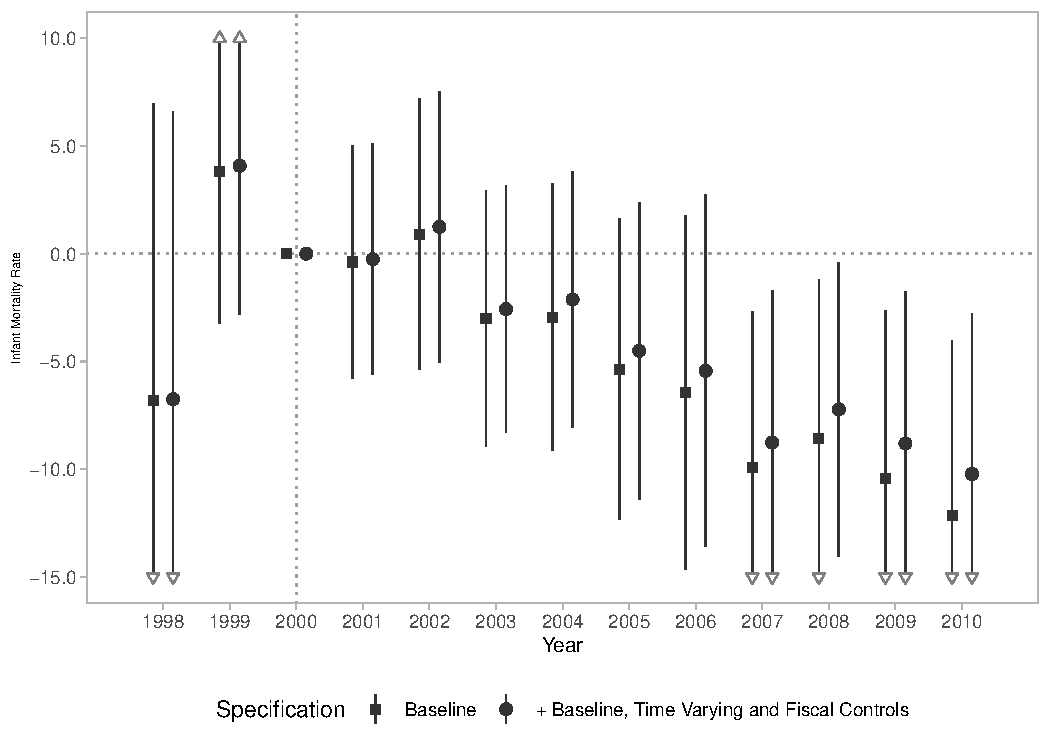
\includegraphics[width=\textwidth]{plots/tx_mi_dist_ec29_baseline_dist_ec29_baseline_15.pdf}
    \end{subfigure}
    \begin{subfigure}{0.32\textwidth}
        \centering
        \caption{\scriptsize Amenable to Primary Care}\label{fig:15b}
        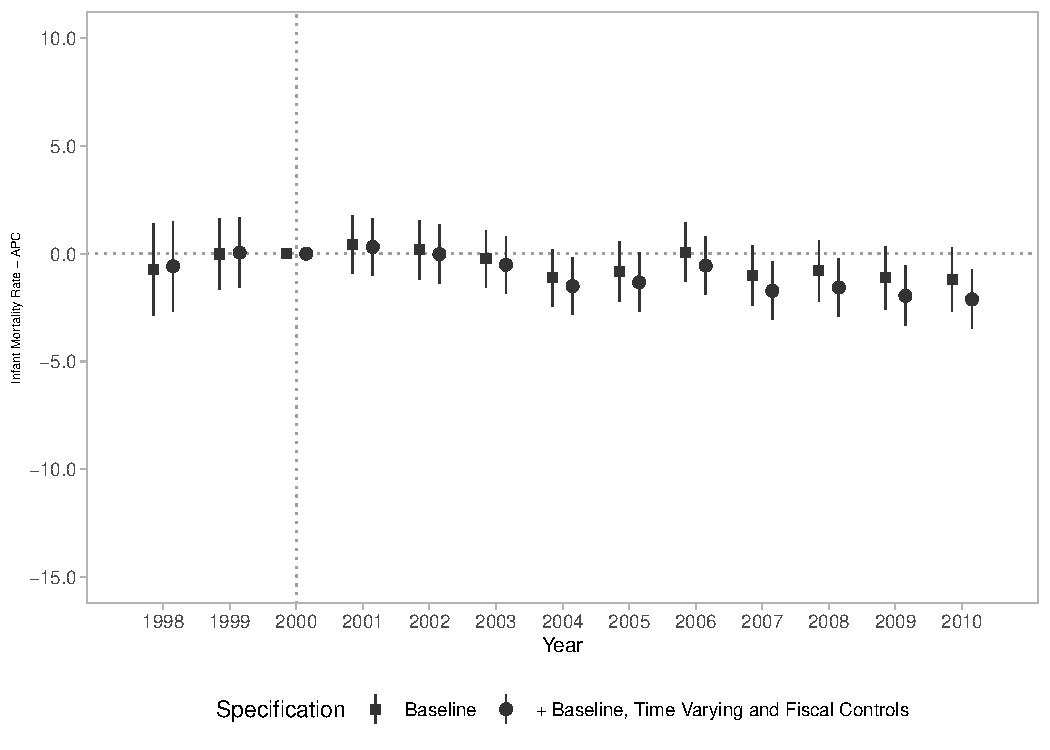
\includegraphics[width=\textwidth]{plots/tx_mi_icsap_dist_ec29_baseline_dist_ec29_baseline_15.pdf}
    \end{subfigure}
    \begin{subfigure}{0.32\textwidth}
        \centering
        \caption{\scriptsize Non-Amenable to Primary Care}\label{fig:15c}
        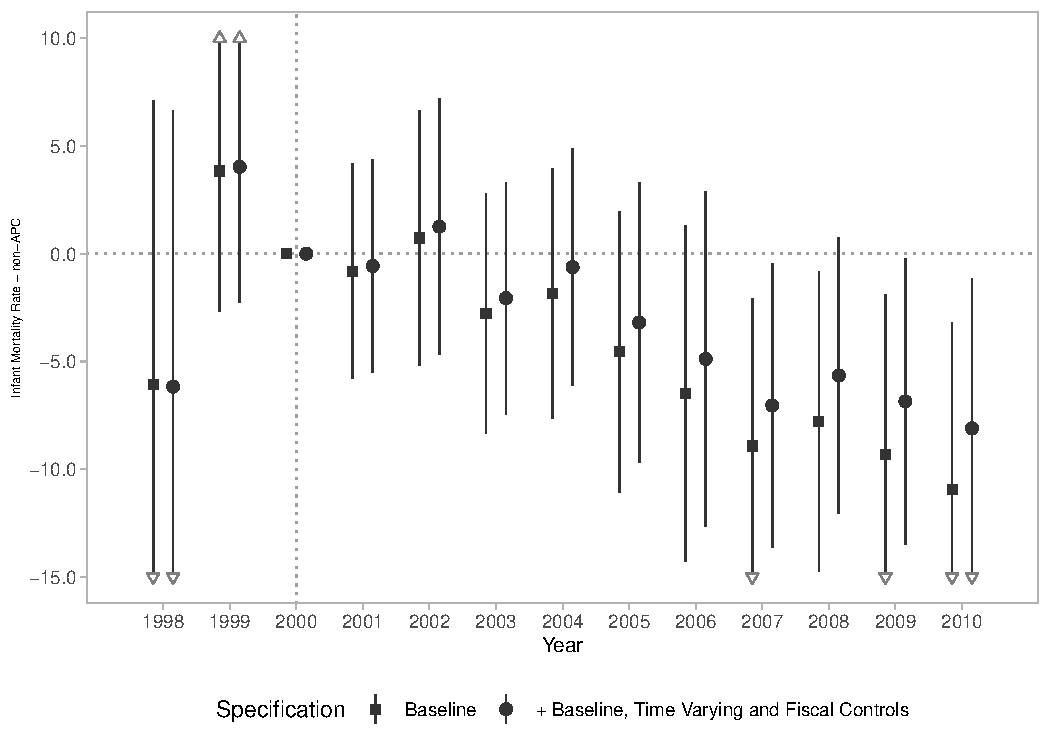
\includegraphics[width=\textwidth]{plots/tx_mi_nicsap_dist_ec29_baseline_dist_ec29_baseline_15.pdf}
    \end{subfigure}
    
    \end{center}
    
        \scriptsize{Notes: The number of observations is 64482. DiD Estimates from Equation \ref{eq:2}. Independent variable is the distance to the EC/29 target in p.p. Square dots represent the baseline model with municipality and state-year fixed effects. Round dots represent fully saturated specification (Column 4 in regression Tables). Lines represent 95\% confidence intervals. Arrows, when present, indicate confidence intervals out of the plot bounds. Standard errors are clustered in the municipality level.}
    
\end{figure}